\chapter{Measurement of LArIAT Electric Field}\label{ch:AppendixB}
The electric field of a LArTPC in the drift volume is a fundamental quantity for the proper functionality of this technology, as it affects almost every reconstructed quantity such as the position of hits or their collected charge. Given its importance, we calculate the electric field for LArIAT with a single line diagram from our HV circuit and we cross check the obtained value with a measurement relying only on TPC data. 

Before getting into the details of the measurement procedures, it is important to explicit the relationship between some  quantities in play. The electric field and the drift velocity ($v_{drift}$) are related as follows 
\begin{equation} v_{drift} = \mu(E_{field},T) E_{field}, \label{eq:vd}
\end{equation}
where $\mu$ is the electron mobility, which depends on the electric field and on the temperature (T). The empirical formula for this dependency is described in ~\cite{WWW} and shown in Figure \ref{fig:EV} for several argon temperatures.

\begin{figure}[htb]
\centering
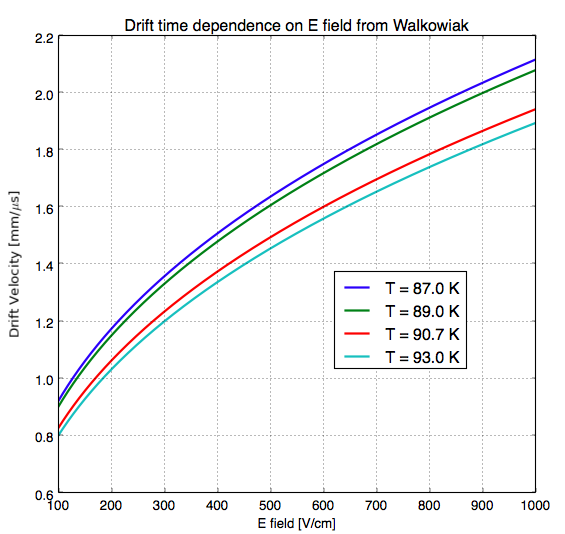
\includegraphics[scale=0.45]{./AppendixB-EField/Images/Walkowiak.png}\\
\caption{Drift velocity dependence on electric field for several temperatures. The slope of the line at any one point represents the electron mobility for that given temperature and electric field.}
\label{fig:EV}
\end{figure}



The relationship between the drift time ($t_{drift}$) and the drift velocity is trivially given by
\begin{equation}
t_{drift} = \Delta x/v_{drift}, \label{eq:drifttime}
\end{equation}
where $\Delta x$ is the distance between the edges of the drift region.
Table \ref{tab:Efields} reports the values of the electric field, drift velocity, and drift times for the smaller drift volumes. 

\begin{table}[]
\centering
\caption{Electric field and drift velocities in LArIAT smaller drift volumes}
\label{tab:Efields}
\begin{tabular}{|l|l|l|}
\hline
& Shield-Induction & Induction-Collection \\ \hline
E$_{field}$ &                 700.63 V/cm        &                892.5  V/cm             \\ \hline
v$_{drift}$ &                   1.73  mm/$\mu$s   &                  1.90 mm/$\mu$s        \\ \hline
t$_{drift}$ &                   2.31  $\mu$s      &                   2.11 $\mu$s          \\ \hline

\end{tabular}
\end{table}

With these basic parameters established, we can now move on to calculating the electric field in the main drift region (between the cathode and the shield plane).

\subsection*{Single line diagram method}
The electric field strength in the LArIAT main drift volume can be determined knowing the voltage applied to the cathode, the voltage applied at the shield plane, and the distance between them. We assume the distance between the cathode and the shield plane to be 470 mm and any length contraction due to the liquid argon is negligibly small ($\sim$2~mm).

The voltage applied to the cathode can be calculated using Ohm's law and the single line diagram shown in Figure \ref{fig:circuit}.  A set of two of filter pots for emergency power dissipation are positioned between the Glassman power supply and the cathode, one at each end of the feeder cable, each with an internal resistance of 40~M$\Omega$.  The output current of the Glassman power supply is then used to determine the electric field strength.  Figure \ref{fig:currentMeasurement} shows an average current of 0.004172 mA from the Glassman power supply.  

\begin{figure}[h]
\centering
\begin{minipage}{0.45\textwidth}
\centering
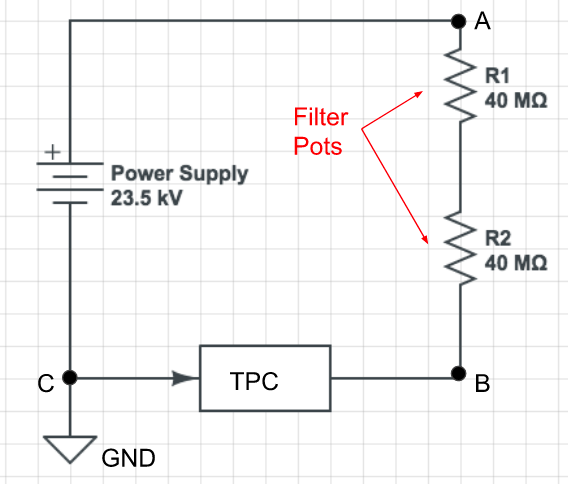
\includegraphics[width=3in]{AppendixB-EField/Images/CircuitLArIAT.png}
\caption{LArIAT HV simple schematics.}
\label{fig:circuit}
\end{minipage}\hfill
\begin{minipage}{0.45\textwidth}
\centering
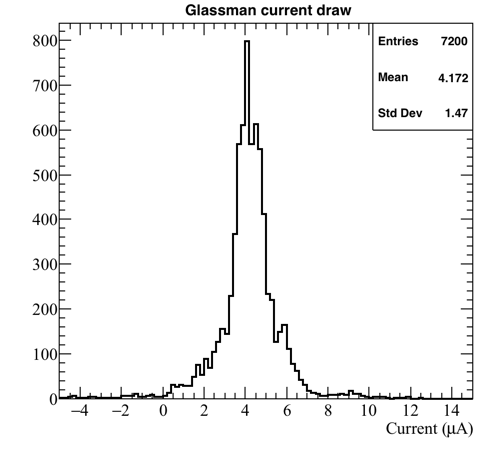
\includegraphics[width=3in]{AppendixB-EField/Images/glassman_current_20160525-30.png}
\caption{Current reading from the Glassman between May 25th and May 30th, 2016 (typical Run-II conditions).}
\label{fig:currentMeasurement}
\end{minipage}
\end{figure}

Using this current, the voltage at the cathode is calculated as
\begin{equation} \label{eq:VBC}
V_{BC}=V_{PS} - (I \times R_{eq}) = -23.5\text{ kV} + ( 0.00417\text{ mA} \times 80\text{ M}\Omega ) = -23.17\text{ kV}, 
\end{equation}
where $I$ is the current and $R_{eq}$ is the equivalent resistor representing the two filter pots. The electric field, drift voltage, and drift time are then calculated to be
\begin{equation}E_{\text{field}} = \frac{V_{BC} - V_{\text{shield}}}{\Delta x} = 486.54\text{ V/cm}
\end{equation}
%\begin{equation}v_{drift} = \mu E_{field} = 1.5097 \textit{ mm/$\mu$s}
%\end{equation}
%\begin{equation}t_{drift} = \frac{\Delta x}{v_{drift}} = 311.316 \textit{ $\mu$s.}
%\end{equation}



\subsection*{E field using cathode-anode piercing tracks}
%%%%%%%%%%%%%%%%%%%%%%%%%%%%%%%%%%%%%%%%%%%%%%%%%%%%%%%%%%%%%%%%%%%%%%%%%%
\begin{figure}[b]
\centering
\begin{minipage}{0.45\textwidth}
\centering
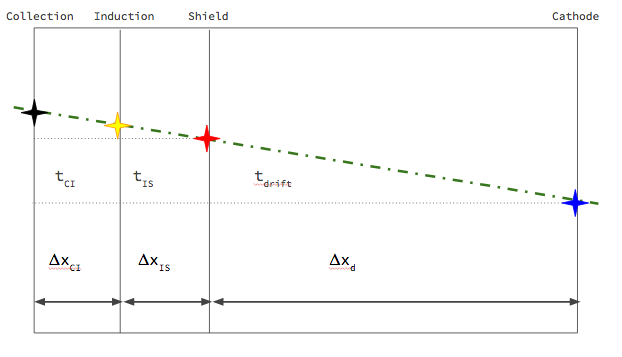
\includegraphics[width=3in]{AppendixB-EField/Images/TPCCrossSectionView.png}
\caption{Pictorial representation of the YX view of the TPC. The distance within the anode planes and between the shield plane and the cathode is purposely out of proportion to illustrate the time difference between hits on collection and induciton. A ACP track is shown as an example.}
\label{fig:Scheme}
\end{minipage}\hfill
\begin{minipage}{0.45\textwidth}
\centering
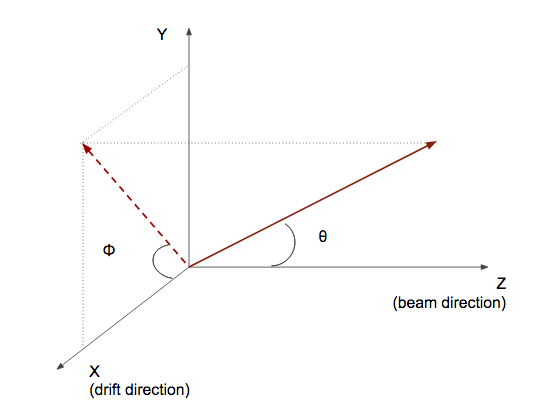
\includegraphics[width=3in]{AppendixB-EField/Images/AngleDef.png}
\caption{Angle definition in the context of LArIAT coordinates system.}
\label{fig:AngleDef}
\end{minipage}
\end{figure}
We devise an independent method to measure the drift time (and consequently drift velocity and electric field) using TPC cathode to anode piercing tracks. We use this method as a cross check to the single line method.
The basic idea is simple:
\begin{itemize}
\item[0.] Select cosmic ray events with only 1 reconstructed track 
\item[1.] Reduce the events to the one contaoning tracks that cross both anode and cathode
\item[2.] Identify the first and last hit of the track
\item[3.] Measure the time difference between these two hits ($\Delta t$).
\end{itemize}
This method works under the assumptions that the time it takes for a cosmic particle to cross the chamber ($\sim$ns) is small compared to the charge drift time ($\sim$ hundreds of $\mu$s).

We choose cosmic events to allow for a high number of anode to cathode piercing tracks (ACP tracks), rejecting  beam  events where the particles travel almost perpendicularly to drift direction. We select events with only one reconstructed track to  maximize the chance of selecting a single crossing muon (no-michel electron). We utilize ACP tracks because their hits span the full drift length of the TPC, see figure \ref{fig:Scheme}, allowing us to define where the first and last hit of the tracks are located in space regardless of our assumption of the electric field. %The definition of the last hit is easy: it is the hit closest to the cathode. The definition of the first hit is a bit more complicated. A track that crosses the anode planes will deposit charge in the small drift volumes (S-I and I-C). The drift time in S-I and I-C region was already calculated in Table \ref{tab:Efields}. This is to say that the position of the first hit matters when calculating the drift time at the microsecond precision. Single hits on the collection plan will not form a 3D object. This means that we can safely exclude that the reconstruction of ACP tracks starts at the cathode plane (black point in figure \ref{fig:Scheme}). %Understanding if the first hit of a track in on the induction or on the shield plan is more complicated. For now, we'll take an uncertainty hit of 2.3 $\mu$s.


One of the main features of this method is that it doesn't rely on the measurement of the trigger time. Since $\Delta t$ is the time difference between the first and last hit of a track and we assume the charge started drifting at the same time for both hits, the measurement of the absolute beginning of drift time $t_0$ is unnecessary. We boost the presence of ACP tracks in the cosmic sample by imposing the following requirements on tracks:

\begin{itemize}
\item vertical position (Y) of first and last hits within $\pm$ 18 cm from TPC center (avoid Top-Bottom tracks) 
\item horizontal position (Z) of first and last hits within 2 and 86 cm from TPC front face (avoid through going tracks) 
\item track length greater than 48 cm (more likely to be crossing)
\item angle from the drift direction (phi in figure \ref{fig:AngleDef}) smaller than 50 deg (more reliable tracking)
\item angle from the beam direction (theta in figure \ref{fig:AngleDef}) grater than 50 deg (more reliable tracking)
\end{itemize}


Tracks passing all these selection requirements are used for the $\Delta t$ calculation.

For each track passing our selection, we loop through the associated hits in order to retrieve the timing information. The analysis is performed separately on hits on the collection plane and induction plane, but lead to consistent results. As an example of the time difference, figures \ref{fig:Run2PosColFit} and \ref{fig:Run2PosIndFit} represent the difference in time between the last and first hit of the selected tracks for Run-II Positive Polarity sample on the collection and induction plane respectively.  We fit with a Gaussian to the peak of the $\Delta t$ distributions to extract the mean drift time and the uncertainty associated with it. The long tail at low $\Delta t$ represent contamination of non-ACP tracks in the track selection.  We apply the same procedure to Run-I and Run-II, positive and negative polarity alike.

   
\begin{figure}[h!]
\begin{minipage}{0.40\textwidth}
\centering
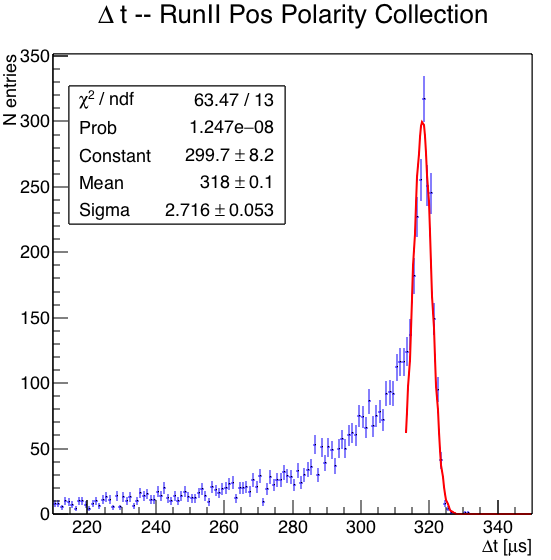
\includegraphics[width=3in]{AppendixB-EField/Images/RunIIPosCol.png}
\caption{Collection plane $\Delta$t fit for Run II positive polarity ACP data  selected tracks.}
\label{fig:Run2PosColFit}
\end{minipage}\hfill
\begin{minipage}{0.40\textwidth}
\centering
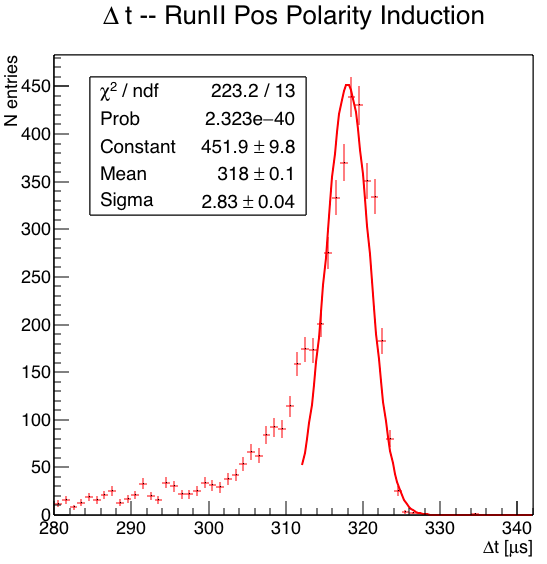
\includegraphics[width=3in]{AppendixB-EField/Images/RunIIPosInd.png}
\caption{Induction plane $\Delta$t fit for Run II positive polarity ACP data  selected tracks.}
\label{fig:Run2PosIndFit}
\end{minipage}
\end{figure}

To convert $\Delta t$ recorded for the hits on the induction plane to the drift time we utilize the formula
\begin{equation}
t_{drift} = \Delta t - t_{S-I}
\end{equation}
where $t_{drift}$ is the time the charge takes to drift in the main volume between the cathode and the shield plane and $t_{S-I}$ is the time it takes for the charge to drift from the shield plane to the induction plane. In Table \ref{tab:Efields} we calculated the drift velocity in the S-I region, thus we can calculate $t_{S-I}$ as 
\begin{equation}
t_{S-I} = \frac{l_{S-I}}{v_{S-I}} = \frac{4 mm}{1.745 mm/ \mu s}
\end{equation}
where $\l_{S-I}$ is the distance between the shield and induction plane and $v_{S-I}$ is the drift velocity in the same region. A completely analogous procedure is followed for the hits on the collection plane, taking into account the time the charge spent in drifting from shield to induction as well as between the induction and collection plane
The value for $\Delta t_{drift}$ , the calculated drift velocity ($v_{drift}$), and corresponding drift electric field for the various run periods is given in Table \ref{tab:deltaTACP} and are consistent with the electric field value calculated with the single line diagram method.

\begin{center}
\begin{table}[htb]
  \begin{center}
    %\resizebox{0.45\textwidth}{!}{%
    \begin{tabular}{|c|c|c|c|}
      \multicolumn{4}{c}{\textbf{Delta t$_{drift}$, drift v and E field with ACP tracks}} \\
      \hline \hline
       Data Period  & $\Delta t_{Drift}$ [$\mu s$] & Drift velocity [mm/$\mu$s] & E field [V/cm] \\
       \hline
       RunI Positive Polarity Induction &  311.1 $\pm$ 2.4   &1.51 $\pm$ 0.01  & 486.6 $\pm$ 21\\
       \hline
       RunI Positive Polarity Collection &  310.9 $\pm$ 2.6 & 1.51 $\pm$ 0.01  &  487.2 $\pm$ 21\\
       \hline
       RunII Positive Polarity Induction &   315.7 $\pm$ 2.8 & 1.49 $\pm$ 0.01 &  467.9 $\pm$ 21\\
       \hline
       RunII Positive Polarity Collection &  315.7 $\pm$ 2.7 & 1.49 $\pm$ 0.01 &  467.9 $\pm$ 21\\
       \hline
       RunII Negative Polarity Induction &   315.9 $\pm$ 2.6 & 1.49 $\pm$ 0.01  & 467.1 $\pm$ 21 \\
       \hline
       RunII Negative Polarity Collection &  315.1 $\pm$ 2.8 & 1.49 $\pm$ 0.01  & 470.3 $\pm$ 21  \\
       \hline
       \hline
       Average Values & 314.1 & 1.50 $\pm$ 0.01 & 474.3 $\pm$ 21 \\
       \hline
       \end{tabular}
    \caption{$\Delta t$ for the different data samples used for the Anode-Cathode Piercing tracks study. }
    \label{tab:deltaTACP}
    \end{center}
\end{table}
\end{center}

%%%%%%%%%%%%%%%%%%%%%%%%%%%%%%%%%%%%%%%%%%%%%%%%%%%%%%%%%%%%



